\section{Code structure}

\castro\ is built upon the \boxlib\ \cpp\ framework.  This provides
high-level classes for managing an adaptive mesh refinement simulation,
including the core data structures we will deal with.

The code structure in the {\tt Castro/} directory is as follows:
\begin{itemize}
\item {\tt constants/}: contains a file of useful constants in CGS units

\item {\tt Docs/}: you're reading this now!

\item {\tt Exec/}: various problem implementations, including:
  \begin{itemize}
  \item {\tt Sedov/}: run directory for the Sedov problem
  \item {\tt Sod/}: run directory for the Sod problem
  \item {\tt KH/}: run directory for the Kelvin-Helmholz problem
  \item $\ldots$
  \end{itemize}

\item {\tt Microphysics/}: contains directories for different default microphysics
  \begin{itemize}
  \item {\tt conductivity/}: the thermal conductivity
  \item {\tt EOS/}: the equation of state
  \item {\tt networks/}: the nuclear reaction networks
  \end{itemize}

\item {\tt Source/}: source code

\item {\tt Util/}: a catch-all for additional things you may need
  \begin{itemize}
  \item {\tt ConvertCheckpoint/}: a tool to convert a checkpoint file to
     a larger domain
  \item $\ldots$
  \end{itemize}


\end{itemize}


\section{Major data structures}

The following data structures are the most commonly encountered when
working in the \cpp\ portions of \castro.  This are all
\boxlib\ data-structures / classes.

\subsection{{\tt Amr}}

This is the main class that drives the whole simulation.  This is 
the highest level in \castro.


\subsection{{\tt AmrLevel} and {\tt Castro} classes}

An {\tt AmrLevel} is a virtual base class provided by \boxlib\ that
stores all the state data on a single level in the AMR hierarchy and
understands how to advance that data in time.

The most important data managed by the {\tt AmrLevel} is an array of
{\tt StateData}, which holds the fluid quantities, etc., in the boxes
that together make up the level.

The {\tt Castro} class is derived from the {\tt AmrLevel}.  It provides
the \castro-specific routines to evolve our system of equations.  Like
the {\tt AmrLevel}, there is one {\tt Castro} object for each level in the
AMR hierarchry.

A lot of the member data in the {\tt Castro} class are static member
variables---this means that they are shared across all instances of
the class.  So, in this case, every level will have the same data.
This is done, in particular, for the values of the runtime parameters,
but also for the {\tt Gravity}, {\tt Diffusion}, and {\tt Radiation}
objects.  This means that those objects cover all levels and are the
same object in each instantiation of the {\tt Castro} class.

\subsection{Floating point data}

Floating point data in the \cpp\ \boxlib\ frame work is declared as
{\tt Real}.  This is {\tt typedef} to either {\tt float} or {\tt
  double} depending on the make variable \makevar{PRECISION}.

\subsection{\bbox\ and \farraybox}

A \bbox\ is simply a rectangular region in space.  It does not hold
data.  In \boxlib, an AMR level has a global index space, with
$(0,0,0)$ being the lower left corner of the domain at that level, and
$(N_x-1, N_y-1, N_z-1)$ being the upper right corner of the domain
(for a domain of $N_x \times N_y \times N_z$ zones).  The location of
any \bbox\ at a level can be uniquely specified with respect to this
global index space by giving the index of its lower-left and
upper-right corners.  Figure~\ref{fig:soft:indexspace} shows an
example of three boxes at the same level of refinement.
\boxlib\ provides other data structures that collect \bbox es together
(e.g., \boxarray), but we will not usually use those directly.

\begin{figure}[t]
\centering
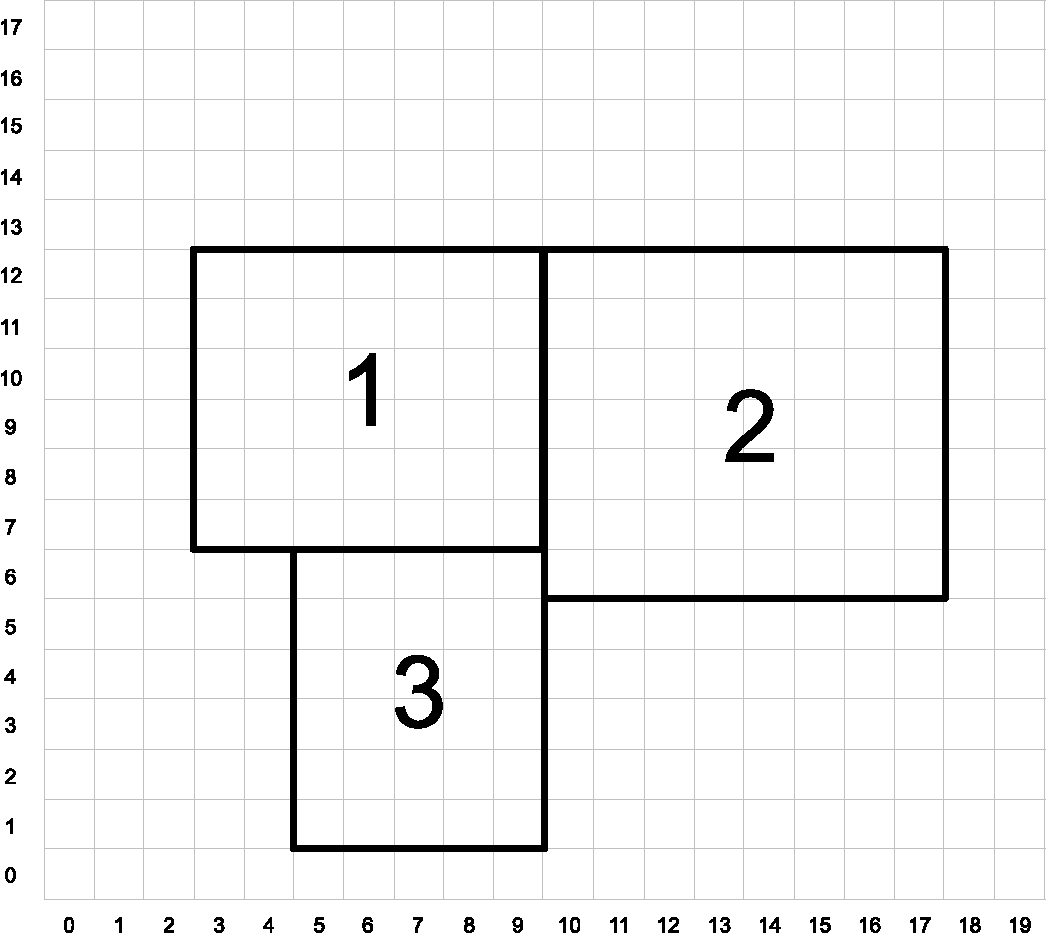
\includegraphics[width=4.0in]{index_grid2}
\caption[Single-level grid structure]
{\label{fig:soft:indexspace} Three boxes that comprise a single level.  At this
  resolution, the domain is 20$\times$18 zones.  Note that the
  indexing in BoxLib starts with $0$.}
\end{figure}


A \farraybox\ or {\em FAB}, for {\em Fortran array box} is a data
structure that contains a \bbox\ locating it in space, as well as a
pointer to a data buffer.  The key part of the \cpp\ \boxlib\ data
structures is that this data buffer can be sent to Fortran, where it
will appear as a {\tt DIM}+1 dimensional array ({\tt DIM} space + 1
component).

Note: \castro\ is complied for a specific dimensionality.


\subsection{\multifab}

A \multifab\ is a collection of the \farraybox s that together make up
a single level of data in the AMR hierarchy.  A \multifab\ can have
multiple components (like density, temperature, ...) as well as a
perimeter of ghost cells to exchange data with neighbors or implement
boundary conditions (this is all reflected in the underlying
\farraybox).

Parallelization in \boxlib\ is done by distributing the FABs across
processors.  Each processor knows which FABs are local to it.  To loop
over all the boxes local to a processor, an \mfiter\ is used (more
on this below).

High-level operations exist on \multifab s to add, subtract, multiply,
etc., them together or with scalars, so you don't need to write out
loops over the data directly.

In \castro, \multifab s are one of the main data structures you will
interact with in the \cpp\ portions of the code.


\subsection{\statedata}

\statedata\ is a class that essentially holds a pair of \multifab s: one
at the old time and one at the new time.  \boxlib\ knows how to
interpolate in time between these states to get data at any
intermediate point in time.  The main data that we care about in
\castro\ (the fluid state, gravitational potential, etc.) will be
stored as \statedata.  Essentially, data is made \statedata\ in
\castro\ if we need it to be stored in checkpoints / plotfiles, and/or
we want it to be automatically interpolated when we refine.

An {\tt AmrLevel} stores an array of \statedata.  We index this array
using integer keys (defined via an {\tt enum} in {\tt Castro.H}).  
The state data is registered with \boxlib\ in \code{Castro\_setup.cpp}.
The current \statedata\ that \castro\ carries is:
\begin{itemize}
\item {\tt State\_Type} : this is the {\tt NUM\_STATE} hydrodynamics
  components that make up the conserved hydrodynamics state (usually
  referred to as $\Ub$ in these notes.  But note that this does 
  not include the radiation energy density.
  
  In Fortran, the components of a FAB derived from {\tt State\_Type}
  is indexed using the integer keys defined in \code{Castro\_nd.F90}
  and stored in \code{meth\_params\_module}, e.g., {\tt URHO}, {\tt UMX},
  {\tt UMY}, ...

  {\tt State\_Type} \multifab s have no ghost cells by default (although, there
  is an option to force them to have ghost cells by setting the parameter
  \runparam{castro.state\_nghost} at runtime.


\item {\tt Rad\_Type} :
\item {\tt PhiGrav\_Type} :
\item {\tt Gravity\_Type} :
\item {\tt PhiRot\_Type} :
\item {\tt Rotation\_Type} :
\item {\tt Source\_Type} :
\item {\tt LS\_State\_Type} :
\item {\tt Reactions\_Type} :
\item {\tt SDC\_Source\_Type} :
\item {\tt SDC\_React\_Type} :
\end{itemize}

We access the multifabs that carry the data of interest by interacting
with the \statedata\ using one of these keys.  For instance:
\begin{lstlisting}
MultiFab& S_new = get_new_data(State_Type);
\end{lstlisting}
gets a pointer to the multifab containing the hydrodynamics state data
at the new time.




\subsection{MFIter}

We iterate over the multifabs using an iterator {\tt MFIter}.  This
iterator knows about the locality of the data---only the boxes on the
processor will be looped over.  An example loop (for the
initialization, from {\tt Castro\_setup.cpp} would be):
\begin{lstlisting}
for (MFIter mfi(S_new); mfi.isValid(); ++mfi)
  {
     const Box& bx      = mfi.validbox();
     const int* lo      = bx.loVect();
     const int* hi      = bx.hiVect();

     if (! orig_domain.contains(bx)) {
        BL_FORT_PROC_CALL(CA_INITDATA,ca_initdata)
          (level, cur_time, lo, hi, ns,
           BL_TO_FORTRAN(S_new[mfi]), dx,
           gridloc.lo(), gridloc.hi());
     }
  }
\end{lstlisting}
Here {\tt BL\_TO\_FORTRAN} is a special \boxlib\ macro that converts the
C++ multifab into a Fortran array, and {\tt BL\_FORT\_PROC\_CALL}
is a BoxLib macro that is used to interface with Fortran routines.
{\tt ++mfi} iterates to the next FArrayBox owned by the MultiFab,
and {\tt mfi.isValid()} returns {\tt false} after we've reached
the last box contained in the MultiFab, terminating the loop.

The corresponding Fortran function will look like:
{\color{red} Need to write the Fortran version here}



\subsection{Boundaries: FillPatch and FillPatchIterator}

FillBoundary -- fills interior ghost cells for an arbitrary multifab

FillPatch works in the case that I have statedata that was defined
with ghost cells already.

FillPatchIterator works on statedata 


\subsection{Boundaries Between Grids}
Boundaries between grids are of two types. The first we call
``fine-fine'', which is two grids at the same level.  Filling ghost
cells at the same level is also part of the fillpatch operation---it's
just a straight copy from ``valid regions'' to ghost cells. The second
type is "coarse-fine", which needs interpolation from the coarse grid
to fill the fine grid ghost cells.  This also happens as part of the
FillPatch operation, which is why arrays aren't just arrays, they're
``State Data'', which means that the data knows how to interpolate
itself (in an anthropomorphical sense).  The type of interpolation to
use is defined in {\tt Castro\_setup.cpp} as well---search for
{\tt cell\_cons\_interp}, for example---that's ``cell conservative
interpolation'', i.e., the data is cell-based (as opposed to node-based
or edge-based) and the interpolation is such that the average of the
fine values created is equal to the coarse value from which they came.
(This wouldn't be the case with straight linear interpolation, for
example.)

A {\tt FillPatchIterator} is used to loop over the grids and fill
ghostcells.  One should never assume that ghostcells are valid.  A key
thing to keep in mind about the {\tt FillPatchIterator} is that you
operate on a copy of the data---the data is disconnected from the
original source.  If you want to update the data in the source,
you need to explicitly copy it back.  Also note: {\tt FillPatchIterator}
takes a multifab, but this is not filled---this is only used to
get the grid layout.  \MarginPar{did I say that right?}

{\color{red}simple example}

Basically, boundary conditions are imposed on ``state variables'' every
time that they're ``fillpatched'', as part of the fillpatch operation.

For example, the loop that calls {\tt CA\_UMDRV} (all the integration stuff) starts with
\begin{lstlisting}
   for (FillPatchIterator fpi(*this, S_new, NUM_GROW,
                              time, State_Type, strtComp, NUM_STATE);
         fpi.isValid(); ++fpi)
   {
     FArrayBox &state = fpi();

     // work on the state FAB
   }
\end{lstlisting}
Here the {\tt FillPatchIterator} is the thing that distributes the
grids over processors and makes parallel ``just work''. This fills the
single patch ``{\tt fpi}'' , which has {\tt NUM\_GROW} ghost cells,
with data of type ``{\tt State\_Type}'' at time ``{\tt time}'',
starting with component {\tt strtComp} and including a total of {\tt
  NUM\_STATE} components.

The way that you tell the code what kind of physical boundary
condition to use is given in {\tt Castro\_setup.cpp}. At the top we
define arrays such as ``{\tt scalar\_bc}'', ``{\tt norm\_vel\_bc}'',
etc, which say which kind of bc to use on which kind of physical
boundary.  Boundary conditions are set in functions like ``{\tt
  set\_scalar\_bc}'', which uses the {\tt scalar\_bc} pre-defined
arrays.

If you want to specify a value at a function (like at an inflow
boundary), there are routines in {\tt Prob\_1d.f90}, for example, which do
that. Which routine is called for which variable is again defined in
{\tt Castro\_setup.cpp}.


\subsection{pArray}



\subsection{Geometry class}

\subsection{ParmParse class}

\subsection{Derived Variables}

\subsection{Error Estimators}


\subsection{Gravity class}


\subsection{Fortran Helper Modules}

There are a number of modules that make data available to the Fortran
side of \castro\ or perform other useful tasks.

\begin{itemize}
\item {\tt prob\_params\_module}:

  This module makes the physical domain lower left and upper right
  coordinates ({\tt problo()} and {\tt probhi}) and problem center
  ({\tt center}) available.

  Here {\tt center} is the center to
  be used for the multipole expansion in gravity, certain diagnostics,
  construction of the radial velocity, etc.  It is not necessarily
  the center of the domain (e.g., for a problem modeling an octant
  of a star, it would be the origin).  This is either set by
  {\tt castro.center} or in the problem's {\tt probinit()}
  subroutine.

  This module also provides the type of physical boundary
  condition in force at each domain edge (and the integer
  keys needed to interpret them).

\item {\tt meth\_params\_module}:

  This module provides the integer keys used to access the state
  arrays for both the conserved variables ({\tt URHO}, {\tt UMX}, $\ldots$)
  and primitive variables ({\tt QRHO}, {\tt QU}, $\ldots$), as well
  as the number of scalar variables.

  It also provides the values of most of the {\tt castro.{\em xxxx}}
  runtime parameters.

\item {\tt model\_parser\_module}:

  This module is built if {\tt USE\_MODELPARSER = TRUE} is set in the
  problem's {\tt GNUmakefile}.  It then provides storage for the an
  initial model and routines to read it in and interpolate onto the
  \castro\ grid.

\item {\tt fundamental\_constants\_module}:

  This provides the CGS values of many physical constants.

\end{itemize}



\section{Setting Up Your Own Problem}

To define a new problem, we create a new directory under {\tt Exec/},
and place in it a {\tt Prob\_2d.f90} file (or {\tt 1d}/{\tt 3d},
depending on the dimensionality of the problem), a {\tt probdata.f90}
file, the {\tt inputs} and {\tt probin} files, and a {\tt
  Make.package} file that tells the build system what problem-specific
routines exist.  Finally, if you need custom boundary conditions, a
{\tt bc\_fill\_2d.f90} (or {\tt 1d}/{\tt 3d}) file is needed.  The
simplest way to get started is to copy these files from an existing
problem.  Here we describe how to customize your problem.

The purpose of these files is:
\begin{itemize}
\item \code{probdata.f90}: this holds the {\tt probdata\_module} Fortran module
  that allocates storage for all the problem-specific runtime parameters that
  are used by the problem (including those that are read from the {\tt probin}
  file.

\item \code{Prob\_?d.f90}: this holds the main routines to
  initialize the problem and grid and perform problem-specific boundary
  conditions:

  \begin{itemize}
  \item {\tt probinit()}:

    This routine is primarily responsible for reading in the {\tt
      probin} file (by defining the {\tt \&fortin} namelist and
    reading in an initial model (usually through the {\tt
      model\_parser\_module}---see the {\tt toy\_convect} problem
    setup for an example).  The parameters that are initialized
    here are those stored in the {\tt probdata\_module}.

  \item \code{ca\_initdata()}:

    This routine will initialize the state data for a single grid.
    The inputs to this routine are:
    \begin{itemize}
    \item {\tt level}: the level of refinement of the grid we are filling

    \item {\tt time}: the simulation time

    \item {\tt lo()}, {\tt hi()}: the integer indices of the box's {\em
      valid data region} lower left and upper right corners.  These
      integers refer to a global index space for the level and
      identify where in the computational domain the box lives.

    \item {\tt nscal}: the number of scalar quantities---this is not typically
      used in \castro.

    \item {\tt state\_l1}, {\tt state\_l2}, ({\tt state\_l3}): the
      integer indices of the lower left corner of the box in each
      coordinate direction.  These are for the box as allocated in memory,
      so they include any ghost cells as well as the valid data regions.

    \item {\tt state\_h1}, {\tt state\_h2}, ({\tt state\_h3}): the
      integer indices of the upper right corner of the box in each
      coordinate direction.  These are for the box as allocated in memory,
      so they include any ghost cells as well as the valid data regions.

    \item {\tt state()}: the main state array.  This is dimensioned as:
\begin{verbatim}
double precision state(state_l1:state_h1,state_l2:state_h2,NVAR)
\end{verbatim}
    (in 2-d), where {\tt NVAR} comes from the {\tt meth\_params\_module}.

    When accessing this array, we use the index keys provided by
    {\tt meth\_params\_module} (e.g., {\tt URHO}) to refer to specific
    quantities

    \item {\tt delta()}: this is an array containing the zone width ($\Delta x$)
      in each coordinate direction: $\mathtt{delta(1)} = \Delta x$,
      $\mathtt{delta(2)} = \Delta y$, $\ldots$.

    \item {\tt xlo()}, {\tt xhi()}: these are the physical coordinates of the
      lower left and upper right corners of the {\em valid region}
      of the box.  These can be used to compute the coordinates of the
      cell-centers of a zone as:
\begin{lstlisting}
  do j = lo(2), hi(2)
     y = xlo(2) + delta(2)*(dble(j-lo(2)) + 0.5d0)
     ...
\end{lstlisting}
     (Note: this method works fine for the problem initialization
     stuff, but for routines that implement tiling, as discussed below,
     {\tt lo} and {\tt xlo} may not refer to the same corner, and instead
     coordinates should be computed using {\tt problo()} from the {\tt
     prob\_params\_module}.)

    \end{itemize}
  \end{itemize}

\item \code{bc\_fill\_?d.f90}:

  These routines handle how \castro\ fills ghostcells {\em
  at physical boundaries} for specific data.  Most problem
  setups won't need to do anything special here, and inclusion
  of this file is optional -- only use it if you need to set
  specific boundary conditions.

  These routines are registered in {\tt Castro\_setup.cpp}, and
  called as needed.  By default, they just
  pass the arguments through to {\tt filcc}, which handles all of
  the generic boundary conditions (like reflecting, extrapolation,
  etc.).  The specific `{\tt fill}' routines can then supply the
  problem-specific boundary conditions, which are typically just
  Dirichlet boundary conditions (usually this means looking to see
  if the {\tt bc()} flag at a boundary is {\tt EXT\_DIR}.  The
  problem-specific code implementing these specific conditions
  should {\em follow} the {\tt filcc} call.

  \begin{itemize}
  \item {\tt ca\_hypfill}:
    This handles the boundary filling for the hyperbolic system.

  \item {\tt ca\_denfill}: At times, we need to fill just the density
    (always assumed to be the first element in the hyperbolic state)
    instead of the entire state.  When the fill patch routine is called
    with {\tt first\_comp = Density} and {\tt num\_comp = 1}, then we
    use {\tt ca\_denfill} instead of {\tt ca\_hypfill}.

    (Note: it seems that this may be used for more than just
    density, but it is only used for tagging and the plotfile)

  \item {\tt ca\_grav?fill}: These routines fill will the ghostcells
    of the gravitational acceleration grids with the gravitational
    acceleration.

    Note: for constant gravity, these routines will never be called.
    For one of the Poisson-type gravities, you only need to do
    something special here if you are implementing an {\tt Interior}
    boundary type (which you can test for by comparing {\tt
    bc(:,:,:)} to {\tt EXT\_DIR}.

    For the other standard physical boundary types, the ghost cell
    filling will be handled automatically by the default {\tt filcc}
    call in these routines.

    The gravitational acceleration in the ghost cells is used during
    the hydrodynamics portion of the code in predicting the
    interface states.

  \item {\tt ca\_reactfill}: This handles boundary filling for
    any {\tt Reactions\_Type} MultiFABs, which are sometimes used to interface
    with the nuclear burning module. It stores the normal state data
    in addition to components for the energy release and species change.

  \end{itemize}

  These routines take the following arguments:
  \begin{itemize}
  \item {\tt adv\_l1}, {\tt adv\_l2}, ({\tt adv\_l3}): the indicies of
    the lower left corner of the box holding the data we are working on.
    These indices refer to the entire box, including ghost cells.

  \item {\tt adv\_h1}, {\tt adv\_h2}, ({\tt adv\_h3}): the indicies of
    the upper right corner of the box holding the data we are working on.
    These indices refer to the entire box, including ghost cells.

  \item {\tt adv()}: the array of data whose ghost cells we are filling.
    Depending on the routine, this may have an additional index refering
    to the variable.

    This is dimensioned as:
\begin{verbatim}
  double precision adv(adv_l1:adv_h1,adv_l2:adv_h2)
\end{verbatim}

  \item {\tt domlo()}, {\tt domhi()}: the integer indices of the lower
    left and upper right corners of the valid region of the {\em entire
    domain}.  These are used to test against to see if we are filling
    physical boundary ghost cells.

    This changes according to refinement level: level-0 will
    range from {\tt 0} to {\tt castro.max\_grid\_size},
    and level-n will range from {\tt 0} to
    $\mathtt{castro.max\_grid\_size} \cdot \prod_n \mathtt{castro.ref\_ratio(n)}$.

  \item {\tt delta()}: is the zone width in each coordinate direction,
    as in {\tt initdata()} above.

  \item {\tt xlo()}: this is the physical coordinate of the lower
    left corner of the box we are filling---including the ghost cells.

    Note: this is different than how {\tt xlo()} was defined in
    {\tt initdata()} above.

  \item {\tt time}: the simulation time

  \item {\tt bc()}: an array that holds the type of boundary conditions
    to enforce at the physical boundaries for {\tt adv}.

    Sometimes it appears of the form {\tt bc(:,:)} and sometimes
    {\tt bc(:,:,:)}---the last index of the latter holds the variable
    index, i.e., density, pressure, species, etc.

    The first index is the coordinate direction and the second index
    is the domain face ({\tt 1} is low, {\tt 2} is hi), so {\tt
    bc(1,1)} is the lower $x$ boundary type, {\tt bc(1,2)} is
    the upper $x$ boundary type, {\tt bc(2,1)} is the lower
    $y$ boundary type, etc.

    To interpret the array values, we test against the quantities
    defined in {\tt bc\_types.fi} included in each subroutine,
    for example, {\tt EXT\_DIR}, {\tt FOEXTRAP}, $\ldots$.  The
    meaning of these are explained below.

  \end{itemize}

\end{itemize}


\section{Boundaries}

\subsection{Physical Boundaries}

The following boundary conditions have already been implemented in
\castro\ See {\tt BoxLib/Src/C\_AMRLib/amrlib/BC\_TYPES.H} for some
more details.
\begin{itemize}
\item {\it Outflow}:
  \begin{itemize}
    \item velocity: {\tt FOEXTRAP}
    \item temperature: {\tt FOEXTRAP}
    \item scalars: {\tt FOEXTRAP}
  \end{itemize}

\item {\it No Slip Wall with Adiabatic Temp}:
  \begin{itemize}
  \item velocity: {\tt EXT\_DIR}, $u=v=0$
  \item temperature: {\tt REFLECT\_EVEN}, $dT/dt=0$
  \item scalars: {\tt HOEXTRAP}
  \end{itemize}

\item {\it No Slip Wall with Fixed Temp}:
  \begin{itemize}
  \item velocity: {\tt EXT\_DIR}, $u=v=0$
  \item temperature: {\tt EXT\_DIR}
  \item scalars: {\tt HOEXTRAP}
  \end{itemize}

\item {\it Slip Wall with Adiabatic Temp}:
  \begin{itemize}
  \item velocity: {\tt EXT\_DIR}, $u_n=0$; {\tt HOEXTRAP}, $u_t$
  \item temperature: {\tt REFLECT\_EVEN}, $dT/dn=0$
  \item scalars: {\tt HOEXTRAP}
  \end{itemize}

\item {\it Slip Wall with Fixed Temp}:
  \begin{itemize}
  \item velocity: {\tt EXT\_DIR}, $u_n=0$
  \item temperature: {\tt EXT\_DIR}
  \item scalars: {\tt HOEXTRAP}
  \end{itemize}

\end{itemize}

Here's definitions of some of the funny-sounding ``all-caps''
words from above:
\begin{itemize}
\item {\tt INT\_DIR}: data taken from other grids or interpolated

\item {\tt EXT\_DIR}: data specified on EDGE (FACE) of bndry

\item {\tt HOEXTRAP}: higher order extrapolation to EDGE of bndry

\item {\tt FOEXTRAP}: first order extrapolation from last cell in interior

\item {\tt REFLECT\_EVEN}: $F(-n) = F(n)$ true reflection from interior cells

\item {\tt REFLECT\_ODD}: $F(-n) = -F(n)$ true reflection from interior cells
\end{itemize}


\subsection{Filling the boundaries}


\section{Parallel I/O}

Both checkpoint files and plotfiles are really directories containing
subdirectories: one subdirectory for each level of the AMR hierarchy.
The fundamental data structure we read/write to disk is a MultiFab,
which is made up of multiple FAB's, one FAB per grid.  Multiple
MultiFabs may be written to each directory in a checkpoint file.
MultiFabs of course are shared across CPUs; a single MultiFab may be
shared across thousands of CPUs.  Each CPU writes the part of the
MultiFab that it owns to disk, but they don't each write to their own
distinct file.  Instead each MultiFab is written to a runtime
configurable number of files N (N can be set in the inputs file as the
parameter \runparam{amr.checkpoint\_nfiles} and \runparam{amr.plot\_nfiles}; the
default is 64).  That is to say, each MultiFab is written to disk
across at most N files, plus a small amount of data that gets written
to a header file describing how the file is laid out in those N files.

What happens is $N$ CPUs each opens a unique one of the $N$ files into
which the MultiFab is being written, seeks to the end, and writes
their data.  The other CPUs are waiting at a barrier for those $N$
writing CPUs to finish.  This repeats for another $N$ CPUs until all the
data in the MultiFab is written to disk.  All CPUs then pass some data
to CPU {\tt 0} which writes a header file describing how the MultiFab is
laid out on disk.

We also read MultiFabs from disk in a ``chunky'' manner, opening only $N$
files for reading at a time.  The number $N$, when the MultiFabs were
written, does not have to match the number $N$ when the MultiFabs are
being read from disk.  Nor does the number of CPUs running while
reading in the MultiFab need to match the number of CPUs running when
the MultiFab was written to disk.

Think of the number $N$ as the number of independent I/O pathways in
your underlying parallel filesystem.  Of course a ``real'' parallel
filesytem should be able to handle any reasonable value of $N$.  The
value {\tt -1} forces $N$ to the number of CPUs on which you're
running, which means that each CPU writes to a unique file, which can
create a very large number of files, which can lead to inode issues.
